\chapter*{Traversée de Chiloe\markboth{Traversée de Chiloe}{}}
\section*{22 février 2015}
6 jours pour traverser l'île de Chiloe en vélo du nord au sud.

 Je commence à descendre par la route principale ce qui permet d'avancer bien car la route est goudronnée et avec des montées raisonnables.
\begin{center} 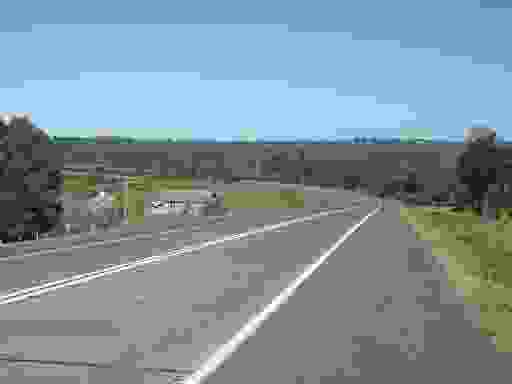
\includegraphics[width=\mywidth]{../wp-content/uploads/2015/02/P2132099.jpg} \end{center}
\vspace{-\topsep}

\pagebreak
 Suite en direction de la côte à l'est, on aperçoit quelques sommets de la cordillère des Andes au loin.
\begin{center} 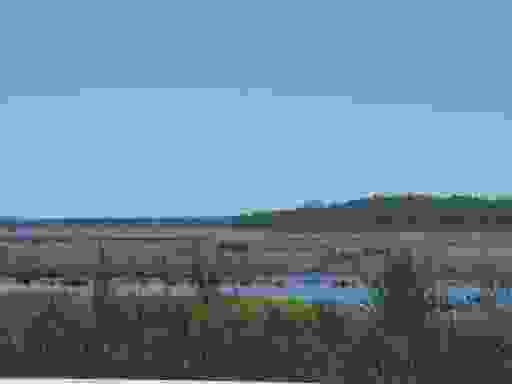
\includegraphics[width=\mywidth]{../wp-content/uploads/2015/02/P2132098.jpg} \end{center}
\begin{center} 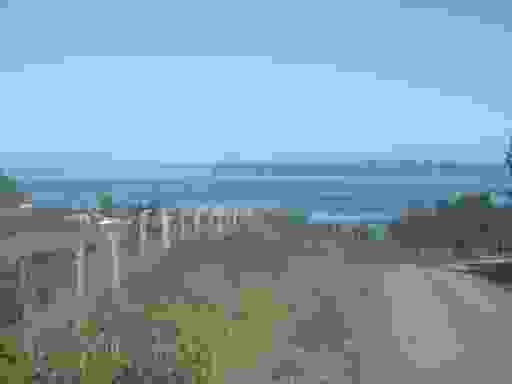
\includegraphics[width=\mywidth]{../wp-content/uploads/2015/02/P2142124.jpg} \end{center}
\vspace{-\topsep}
\vspace{-3mm}

\pagebreak
 Visite d'un petit îlot :
\begin{center} 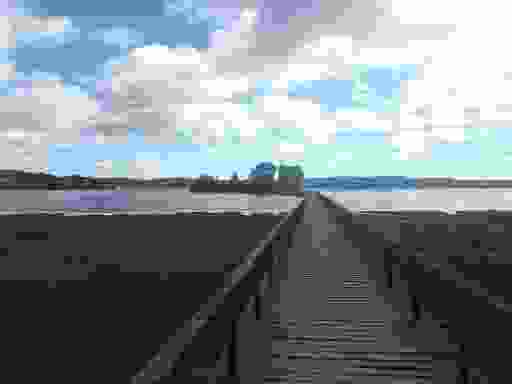
\includegraphics[width=\mywidth]{../wp-content/uploads/2015/02/P2142106.jpg} \end{center}
\begin{center} 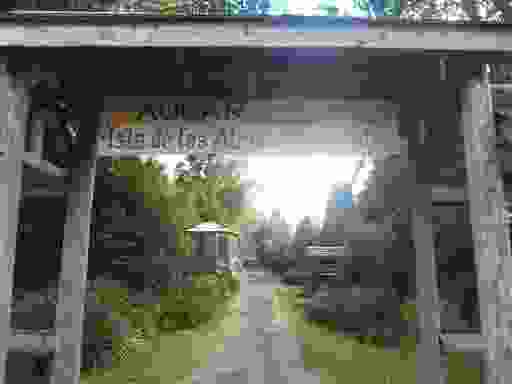
\includegraphics[width=\mywidth]{../wp-content/uploads/2015/02/P2142108.jpg} \end{center}
\vspace{-\topsep}
\vspace{-3.25mm}

\pagebreak
~
\begin{center} 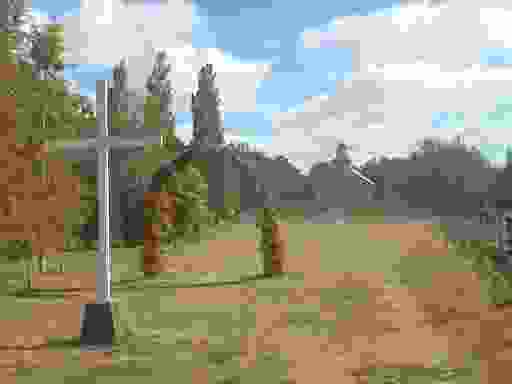
\includegraphics[width=\mywidth]{../wp-content/uploads/2015/02/P2142109.jpg} \end{center}
\begin{center} 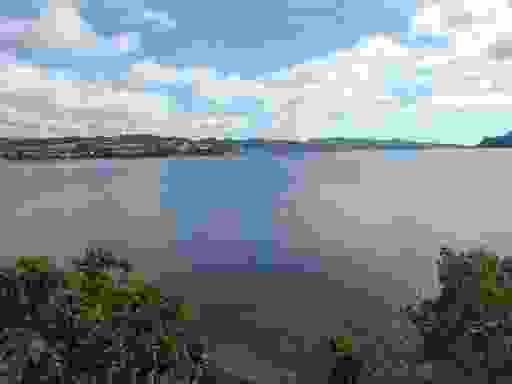
\includegraphics[width=\mywidth]{../wp-content/uploads/2015/02/P2142110.jpg} \end{center}
\vspace{-\topsep}
\vspace{-3.25mm}

\pagebreak
 Passage par une partie de la route des églises de Chiloe, plusieurs d'entre elles sont au patrimoine de l'Unesco.

 \'Eglise de Colo, 3km de piste aller-retour super raide pour y arriver, ça se mérite !

\begin{center} 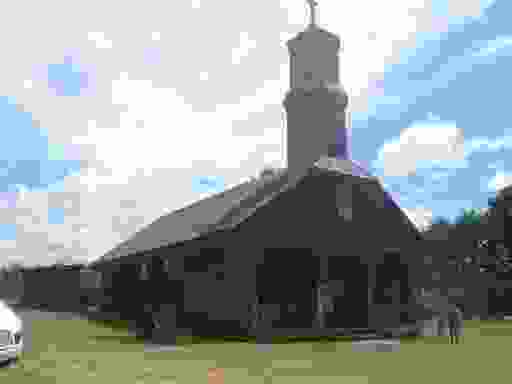
\includegraphics[width=\mywidth]{../wp-content/uploads/2015/02/P2142113.jpg} \end{center}

 \'Eglise de Castro :
\begin{center} 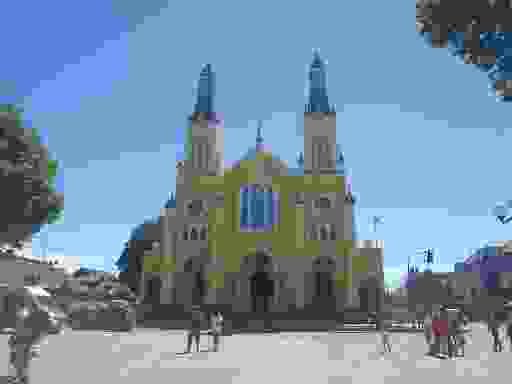
\includegraphics[width=\mywidth]{../wp-content/uploads/2015/02/P2152142.jpg} \end{center}

 \'Eglise de Nercon :
\begin{center} 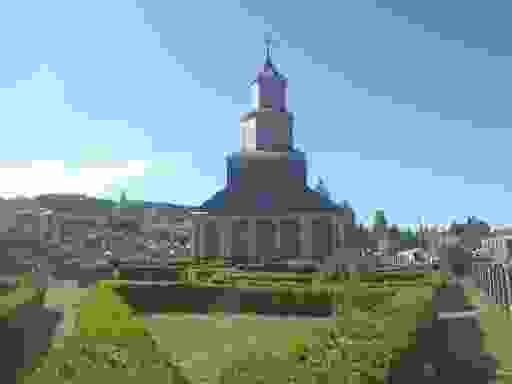
\includegraphics[width=\mywidth]{../wp-content/uploads/2015/02/P2152150.jpg} \end{center}

 Après je ne les ai pas toutes vues, il y en a une vingtaine au total.

 Passage par une cascade sympathique :
\begin{center} 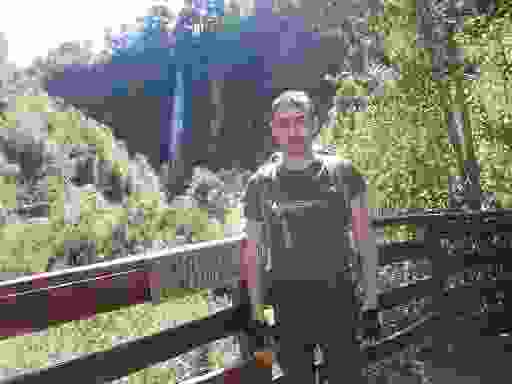
\includegraphics[width=\mywidth]{../wp-content/uploads/2015/02/P2142119.jpg} \end{center}

 Juste avant d´arriver à Castro, la capitale de l´île je me fais rattraper par Jérémy que j´avais croisé à Ancud. Il voyage en vélo depuis 2 ans et demi, il a déjà parcouru la route entre terre de feu et le Canada. Il est revenu dans le sud pour faire quelques endroits qu´il ne connait pas encore !
\begin{center} 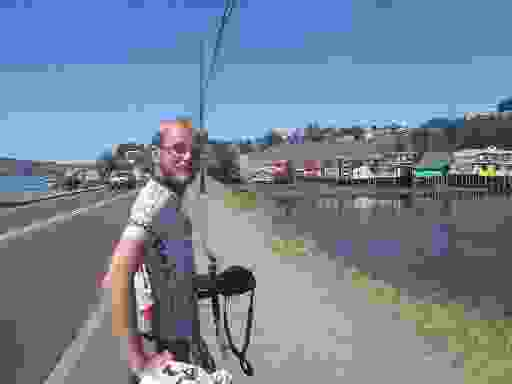
\includegraphics[width=\mywidth]{../wp-content/uploads/2015/02/P2152135.jpg} \end{center}

 Puisque nous allons tous les 2 vers le sud de l´île, nous continuons la route ensemble.

 Castro et ses maisons sur pilotis :
\begin{center} 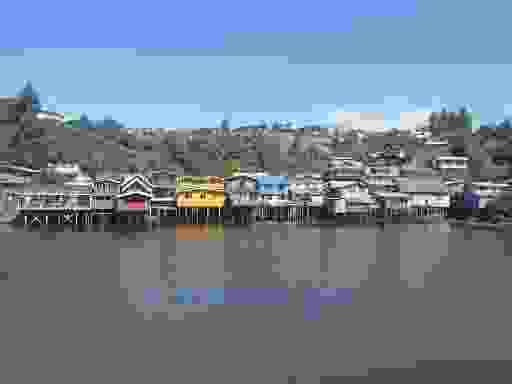
\includegraphics[width=\mywidth]{../wp-content/uploads/2015/02/P2152133.jpg} \end{center}
\vspace{-\topsep}

\pagebreak
~\\
\begin{center} 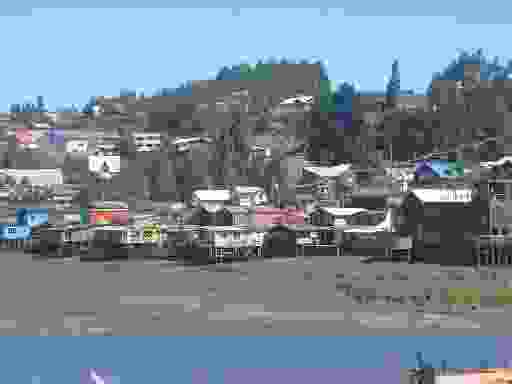
\includegraphics[width=\mywidth]{../wp-content/uploads/2015/02/P2152146.jpg} \end{center}

~

 Je fais bien du vélo ici :\\
\begin{center} 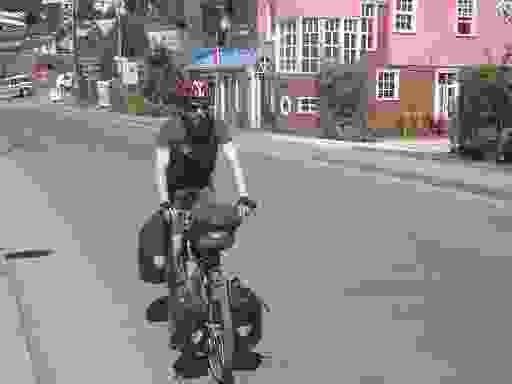
\includegraphics[width=\mywidth]{../wp-content/uploads/2015/02/P2152141.jpg} \end{center}
\vspace{-\topsep}

\pagebreak
 Petite fête locale avec de la musique et des spécialités culinaires :
\begin{center} 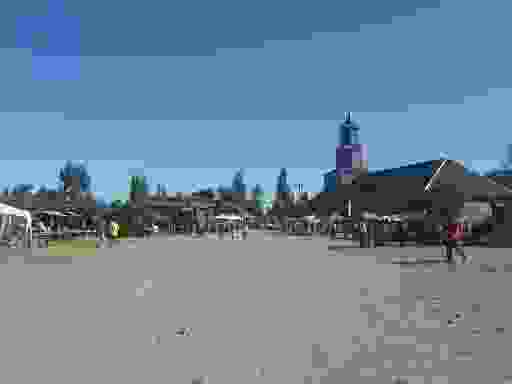
\includegraphics[width=\mywidth]{../wp-content/uploads/2015/02/P2152151.jpg} \end{center}

 Après Castro, nous repartons vers la côte Pacifique et le parc national de Chiloe.

 La route longe un beau lac, l'occasion de se rafraîchir.
\begin{center} 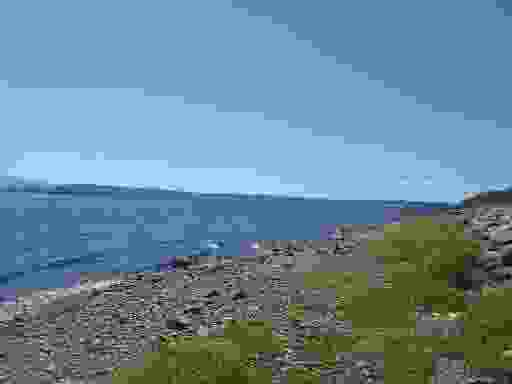
\includegraphics[width=\mywidth]{../wp-content/uploads/2015/02/P2162156.jpg} \end{center}
\vspace{-\topsep}

\pagebreak
~
\begin{center} 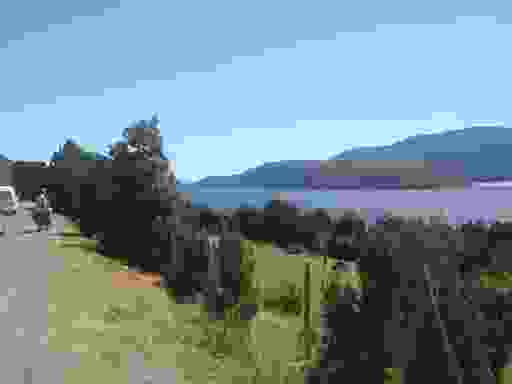
\includegraphics[width=\mywidth]{../wp-content/uploads/2015/02/P2162158.jpg} \end{center}
~\\

~
\begin{center} 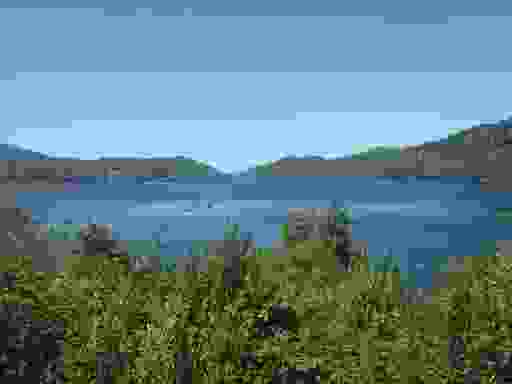
\includegraphics[width=\mywidth]{../wp-content/uploads/2015/02/P2162161.jpg} \end{center}
\vspace{-\topsep}

\pagebreak
 Plage immense au bord du pacifique :
\begin{center} 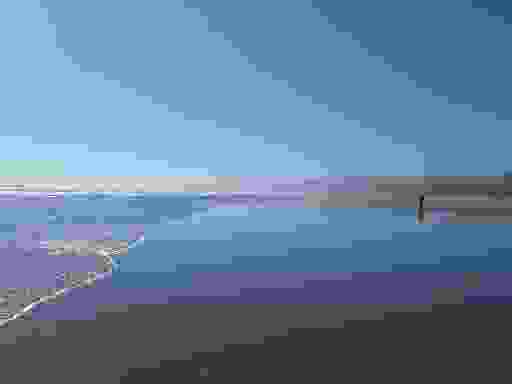
\includegraphics[width=\mywidth]{../wp-content/uploads/2015/02/P2162164.jpg} \end{center}

 Bivouac à quelques mètres de la plage :
\begin{center} 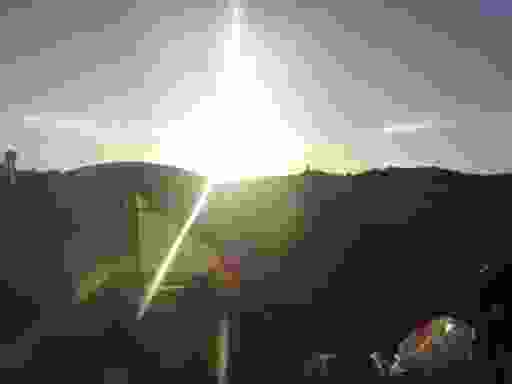
\includegraphics[width=\mywidth]{../wp-content/uploads/2015/02/P2172173.jpg} \end{center}
\vspace{-\topsep}

\pagebreak
~
\begin{center} 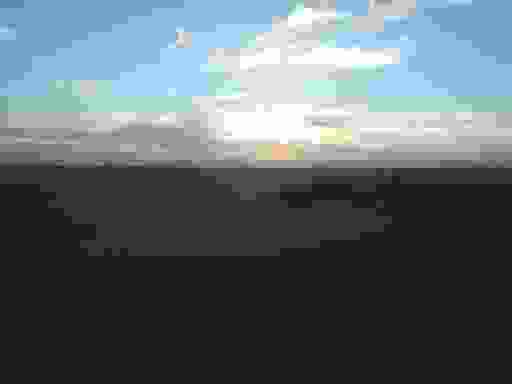
\includegraphics[width=\mywidth]{../wp-content/uploads/2015/02/P2172175.jpg} \end{center}
~
\begin{center} 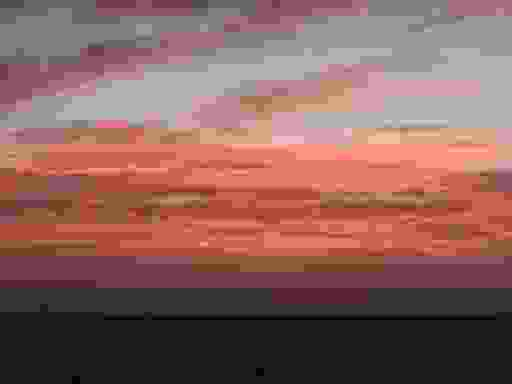
\includegraphics[width=\mywidth]{../wp-content/uploads/2015/02/P2172180.jpg} \end{center}
\vspace{-\topsep}

\pagebreak
 Balade dans le parc national qui contient des forêts très denses et à la végétation particulière :
\begin{center} 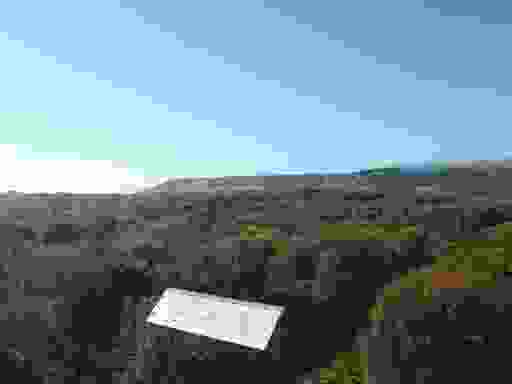
\includegraphics[width=\mywidth]{../wp-content/uploads/2015/02/P2162167.jpg} \end{center}
\begin{center} 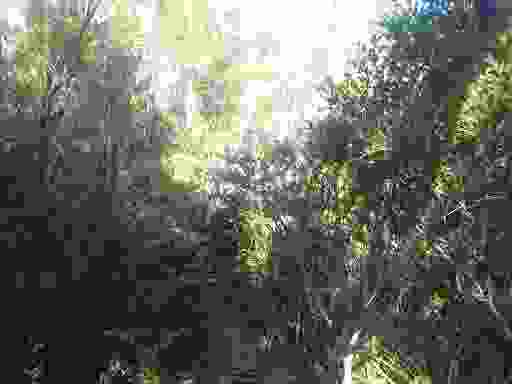
\includegraphics[width=\mywidth]{../wp-content/uploads/2015/02/P2162169.jpg} \end{center}
\vspace{-\topsep}
\vspace{-2.75mm}

\pagebreak
  Dernier bivouac avant de quitter Chiloe :
\begin{center} 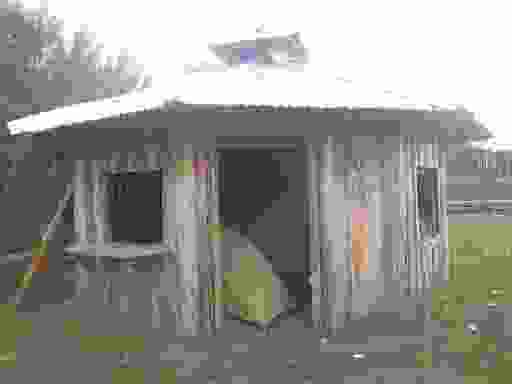
\includegraphics[width=\mywidth]{../wp-content/uploads/2015/02/P2172189.jpg} \end{center}

 Et encore quelques spécialités locales sur la route.

 Les empanadas, il y en a partout avec différentes garnitures, viande, fromage, légumes...
\begin{center} 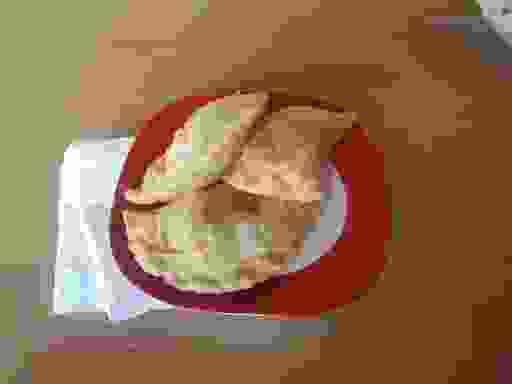
\includegraphics[width=\mywidth]{../wp-content/uploads/2015/02/P2142116.jpg} \end{center}
\vspace{-\topsep}

\pagebreak
 Le Curanto, typique de Chiloe, coquillages, saucisse, porc, pomme de terre et fèves, le tout cuit dans des pierres chaudes.
 \vfill
 \begin{center} 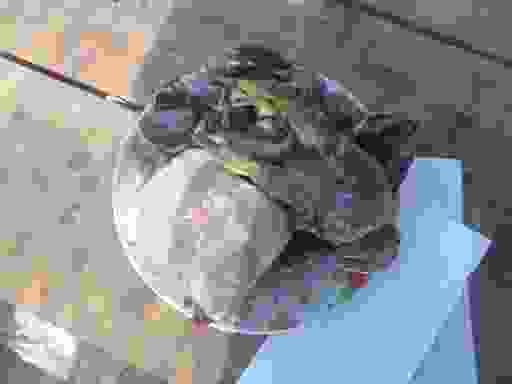
\includegraphics[width=\mywidth]{../wp-content/uploads/2015/02/P2152152.jpg} \end{center}

\vfill
 Le Mote con Huesilla, boisson sucrée avec une pêche et des grains de blé au fond.
 \vfill
\begin{center} 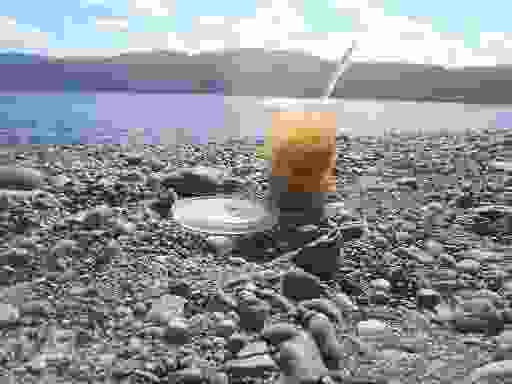
\includegraphics[width=\mywidth]{../wp-content/uploads/2015/02/P2172183.jpg} \end{center}
\vspace{-\topsep}
\vspace{-0.75mm}